\documentclass{article}
\usepackage{fontspec}

% Used to embed Sage code in latex
%\usepackage{sagetex}


% Math Environment
\usepackage{euler}        % Euler font
\usepackage{amsmath}      % Math macros
\usepackage{amssymb}      % Math symbols
\usepackage{unicode-math} % Unicode support

% Physics Environment
\usepackage{physics}


\usepackage[makeroom]{cancel} % Used to cancel terms in algebraic equations
\usepackage{ulem} % Different underline environments
\usepackage{polynom} %Polynomial long division

% Typesetting Rules
\setlength\parindent{0em}
\setlength\parskip{0.618em}
\usepackage[a4paper,lmargin=1in,rmargin=1in,tmargin=1in,bmargin=1in]{geometry}
\setmainfont[Mapping=tex-text]{Helvetica Neue LT Std 45 Light}

% Common Macros
\newcommand\N{\mathbb{N}}
\newcommand\Z{\mathbb{Z}}
\newcommand\Q{\mathbb{Q}}
\newcommand\R{\mathbb{R}}
\newcommand\C{\mathbb{C}}
\newcommand\A{\mathbb{A}}
\def\res{\mathop{\text{Res}}\limits}

% Color
\usepackage[dvipsnames]{xcolor}
\usepackage{pagecolor}
% \definecolor{DeepMossGreen}{HTML}{394820}
% \pagecolor{DeepMossGreen}
% \color{Goldenrod}

\usepackage{graphicx}

\newcommand*\interior[1]{#1^{\mathsf{o}}}

\begin{document}

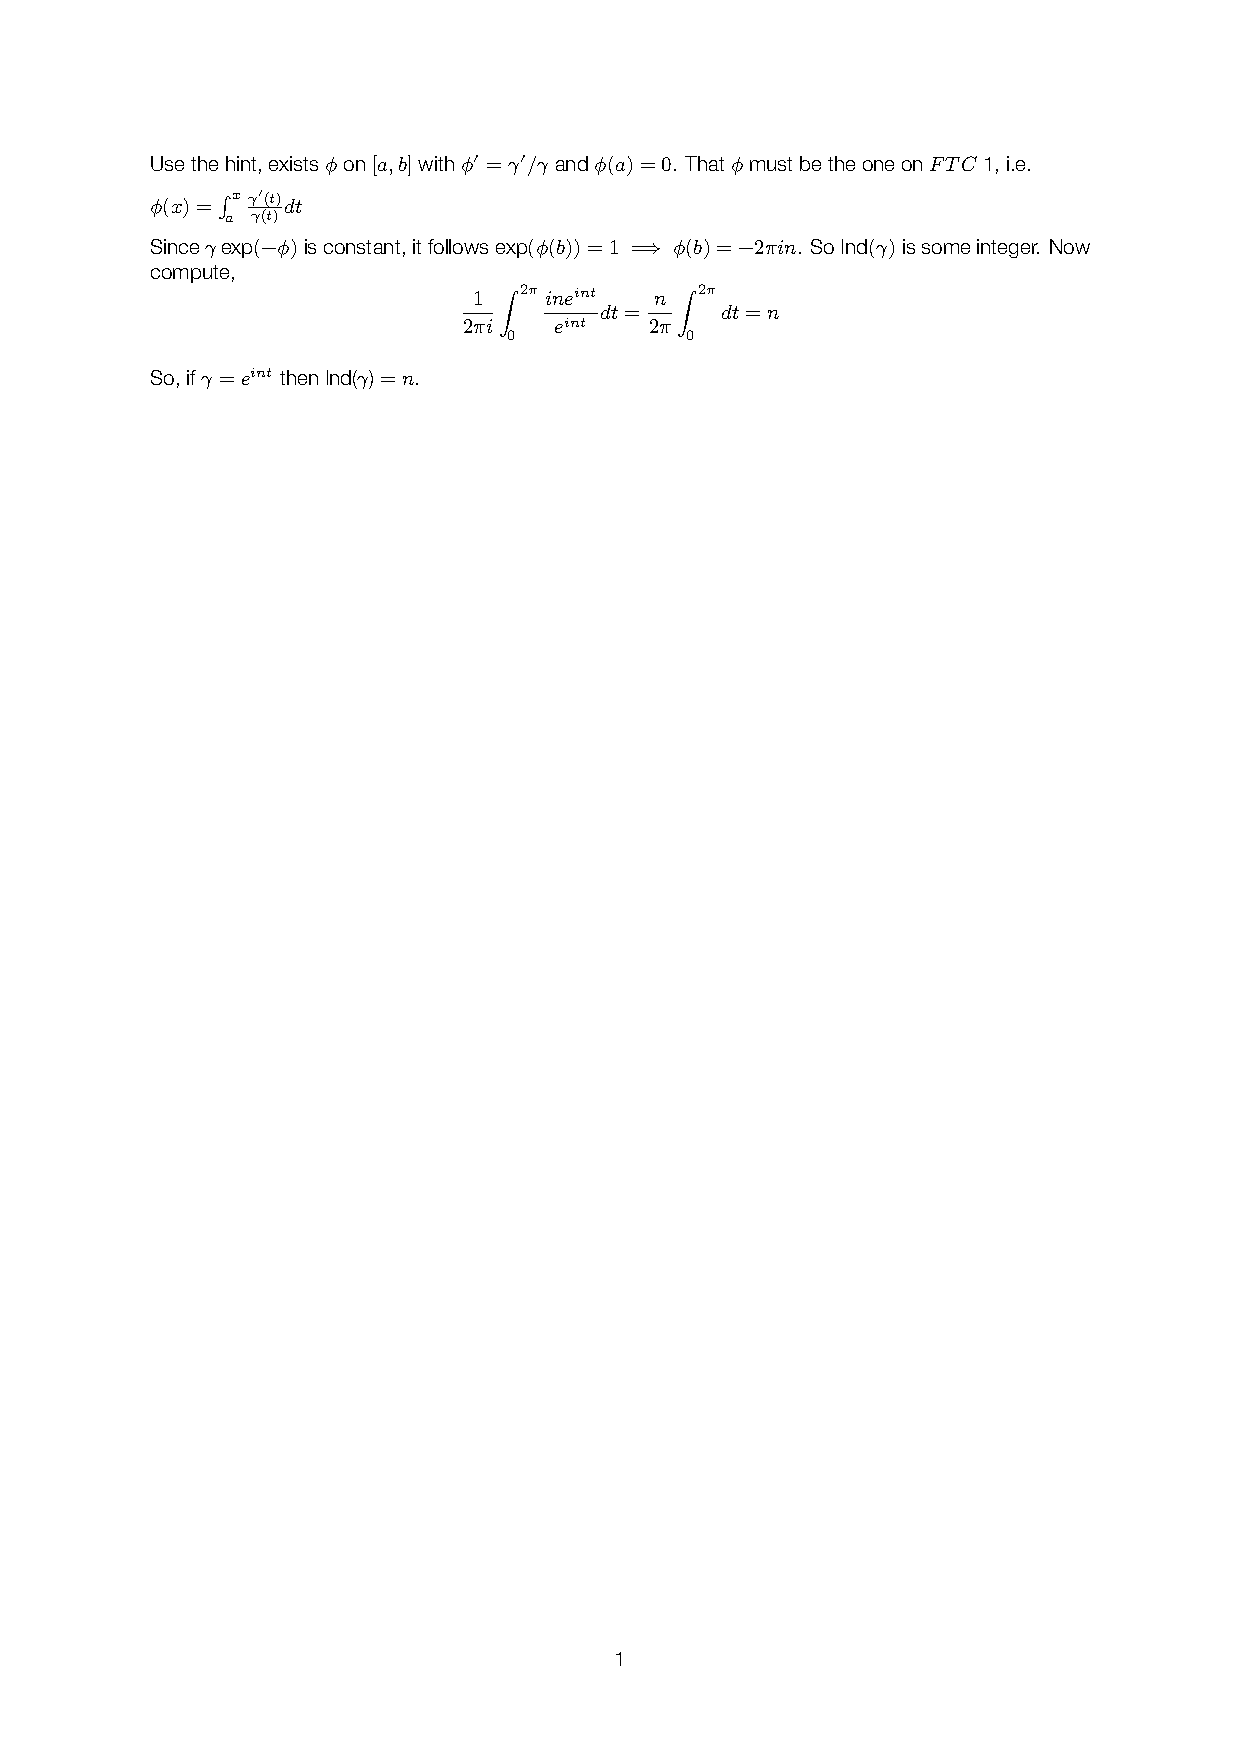
\includegraphics[width=\textwidth]{q3.png}

\uwave{pf.}

By, Proposition 5.1, in \textit{Introduction to Topological
  Manifolds}, by J.M. Lee, GTM 202, pp. 128-129.  $H\subset \R^k$ is a
compact convex set with non-empty interior it is homeomorphic to $\overline{B}^k$ the
closed unit ball centered at the origin,
with the homeomorphism $\phi$ mapping $\partial H\rightarrow S^{k-1} =
\partial B^k$. Let $I^k =\{\vb{x}\in \R^k|,\ -1 \leq x_i\leq 1,\,
1\leq i \leq k\}$, then since $I^k$ is also a compact convex set with
non-empty interior it is
homeomorphic to $\overline{B}^k$,
with the homeomorphism $\psi$ mapping $\partial I^k\rightarrow S^{k-1} =
\partial B^k$. Then $\psi^{-1}\circ \phi$ is a homeomorphism between
$H$ and $I^k$, that is a contiuous bijection from $\partial H$ to $\partial I^k$.

Since $\forall \varepsilon >0: S^{k-1} \subset
D^{k-1}_{1+\varepsilon}(\vb{0})\backslash
D^{k-1}_{1-\varepsilon}(\vb{0})\implies 0\leq \mu(S^{k-1}) \leq \mu(D^{k-1}_{1+\varepsilon}(\vb{0})\backslash
D^{k-1}_{1-\varepsilon}(\vb{0})) = 0$.

So, $\mu(S^{k-1}) = 0$, see \textit{Fractals and Self-similarity},
Hutchinson, 1981, pp. 719-720.

Therefore, by the continuity of $\psi^{-1}$, $\mu(\partial I^k) = 0.$

Then for a function $f$ that's continuous on $H$, we can define
\[\int_H f = \int_{I^k} (\phi^{-1} \circ \psi \circ f)|J_{\phi^{-1}\circ\psi}|\]

And, we can approximate $f$ by a continuous function $F$ on $\R^k$, so
that, for all $\varepsilon > 0$,
\[\bigg|\int_H F - \int_H f\bigg| < \varepsilon.\]

Then, we can apply theorem 10.4, as
\[\int_{H} F = \int_{I^k}  (\phi^{-1} \circ \psi \circ F)|J_{\phi^{-1}\circ\psi}|,\]
is independent of the order of integration.

So that $\int_H f$ is independent of the order of integration. $\quad \blacksquare$

\end{document}




%%% Local Variables:
%%% mode: latex
%%% TeX-master: t
%%% End:
